\chapter{Katalisis Homogen dalam Industri}\label{ch:b3:homogeneous-catalysis}

Sebagian besar asam asetat dunia, bahan baku vinil asetat, selulosa asetat,
dan asam tereftalat murni untuk botol plastik, dibuat dari metanol dan karbon
monoksida di beberapa pabrik yang sangat besar. Di setiap pabrik itu, sebuah
kompleks rodium atau iridium yang terlarut dalam konsentrasi rendah di dalam
cairan reaksi berputar ribuan kali per jam, selama bertahun-tahun. Kimia
sejenis menghidrogenasi, menambahkan CO dan hidrogen pada alkena, menukar
ujung-ujung ikatan rangkap, menyambung cincin aromatik, dan membuat polietilena
serta polipropilena hingga jutaan ton. Bab ini membaca siklus katalitik
proses-proses industri utama dengan perangkat \cref{ch:b3:organometallic-bonding}:
penghitungan elektron, bilangan oksidasi, tahap penentu laju, dan simetri
katalis yang menentukan struktur sebuah polimer.

\begin{recall}
Jilid Tahun 2 memperkenalkan tahap-tahap elementer reaksi organologam
(adisi oksidatif, eliminasi reduktif, insersi migrasi, eliminasi
$\beta$-hidrida, transmetalasi), siklus katalitik, prakatalis, bilangan perputaran
dan frekuensi perputaran, serta membaca siklus hidrogenasi, \omterm{def:b3:homogeneous-catalysis:hydroformylation}{hidroformilasi}, dan
kopling silang; jilid itu juga mendefinisikan taktisitas dan polimerisasi pertumbuhan rantai,
konversi, dan selektivitas. \Cref{ch:b3:organometallic-bonding} menghitung
elektron dan menjelaskan ligan karbonil dan \omterm{def:b3:organometallic-bonding:carbene}{karbena};
\cref{ch:b3:complex-kinetics} memberikan kinetika kejenuhan;
\cref{ch:b3:point-groups} \omterm{def:b3:point-groups:operation}{unsur-unsur simetri} molekul.
\end{recall}

\begin{omfigure}
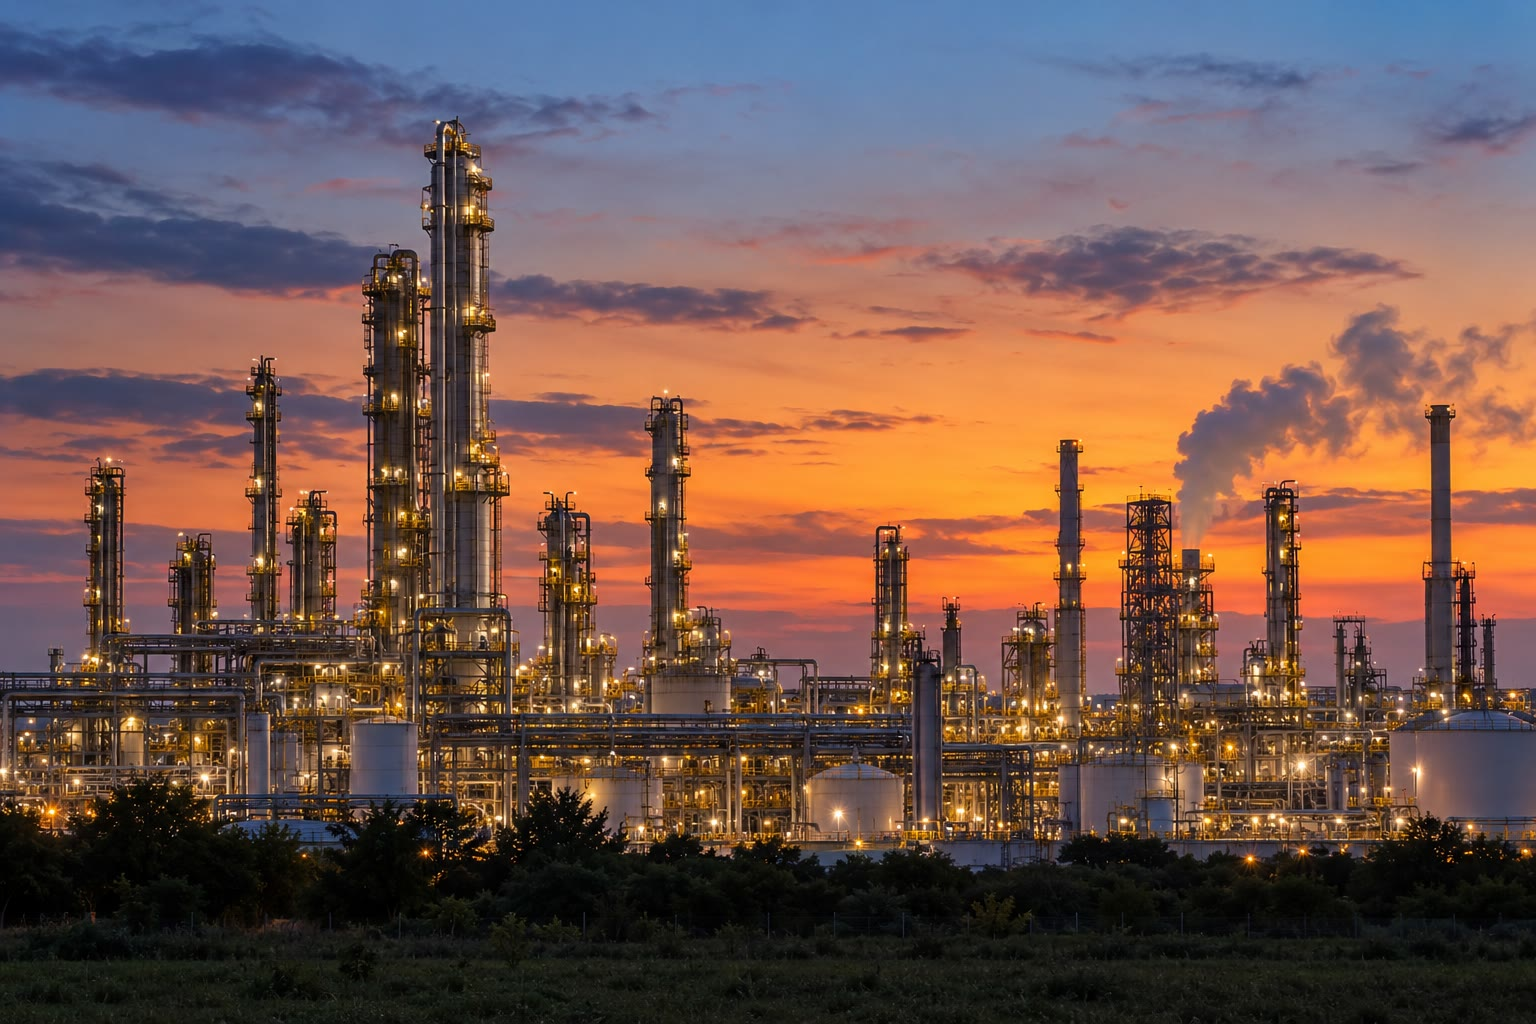
\includegraphics[width=0.6\linewidth]{images/book4/ai/b3-21-chemical-plant.jpg}

{\small Sebuah pabrik kimia besar pada senja hari. Dalam satuan \omterm{def:b3:homogeneous-catalysis:carbonylation}{karbonilasi},
katalisnya adalah kompleks logam yang terlarut dalam cairan reaksi; sebagian
besar pabrik itu bertugas memisahkan dan mendaur ulang.}
\end{omfigure}

\section{Hidrogenasi}

\begin{method}[Membaca siklus katalitik]\label{met:b3:homogeneous-catalysis:read-cycle}
\begin{enumerate}
  \item Pada setiap spesies, hitunglah elektron valensinya dan berikan bilangan
        oksidasi serta $d^n$ logamnya.
  \item Namailah setiap tahap (pelepasan atau penambahan ligan, adisi oksidatif,
        insersi, eliminasi) dan periksalah bahwa hitungannya berubah seperti yang dituntut tahap itu
        (adisi oksidatif: $+2$ pada bilangan oksidasi dan pada jumlah elektron).
  \item Kenali keadaan istirahat (spesies yang menumpuk) dan tahap penentu
        laju; hukum lajunya mengikuti dari prakesetimbangan-prakesetimbangan
        di antara keduanya.
\end{enumerate}
\end{method}

\begin{omfigure}
\begin{tikzpicture}[font=\small, >=Stealth]
  \node (a) at (90:2.3) {\ce{RhCl(PPh3)2} \ (14, Rh$^{\mathrm I}$)};
  \node (b) at (0:3.0) {\ce{RhClH2(PPh3)2} \ (16, Rh$^{\mathrm{III}}$)};
  \node (c) at (-90:2.3) {\ce{RhClH2(RCH=CH2)(PPh3)2} \ (18)};
  \node (d) at (180:3.1) {\ce{RhClH(CH2CH2R)(PPh3)2} \ (16)};
  \draw[->, thick] (a) to[bend left=22] node[midway, above right, font=\scriptsize] {$+\,\ce{H2}$, adisi oksidatif} (b);
  \draw[->, thick] (b) to[bend left=22] node[midway, below right, font=\scriptsize] {$+$ alkena} (c);
  \draw[->, thick] (c) to[bend left=22] node[midway, below left, font=\scriptsize] {insersi migrasi} (d);
  \draw[->, thick] (d) to[bend left=22] node[midway, above left, font=\scriptsize, align=right] {eliminasi reduktif:\\ $-$ alkana} (a);
  \node[anchor=south] (p) at (90:3.4) {\ce{RhCl(PPh3)3} \ (16, prakatalis)};
  \draw[<->, black!50] (p) -- (a) node[midway, right, font=\scriptsize] {$\mp\,\ce{PPh3}$};
\end{tikzpicture}

{\small Siklus hidrogenasi alkena yang disederhanakan dengan katalis Wilkinson
(jumlah elektron valensi dalam kurung). Lepasnya sebuah fosfina membuka sebuah situs;
siklus itu menambahkan hidrogen, mengikat alkena, menyisipkannya ke dalam ikatan Rh--H, dan
mengeliminasi alkana.}
\end{omfigure}

\begin{proposition}[Kinetika Wilkinson]\label{prop:b3:homogeneous-catalysis:wilkinson-rate}
Jika $\ce{RhClL3} \rightleftharpoons \ce{RhClL2} + \mathrm L$ ($K_1$) dan $\ce{RhClL2} + \ce{H2} \rightleftharpoons \ce{RhClH2L2}$ ($K_2$) merupakan kesetimbangan
yang cepat dan reaksi dihidrida dengan alkena (tetapan laju $k$)
merupakan tahap penentu laju,
\[
  v = \frac{kK_1K_2[\mathrm{Rh}]_{\mathrm{tot}}[\ce{H2}][\text{alkena}]}{[\mathrm L] + K_1 + K_1K_2[\ce{H2}]},
\]
yang jenuh terhadap hidrogen dan diinhibisi oleh fosfina L yang ditambahkan.
\end{proposition}

\begin{proof}
$[\ce{RhClL2}] = K_1[\ce{RhClL3}]/[\mathrm L]$ dan $[\ce{RhClH2L2}] = K_2[\ce{H2}][\ce{RhClL2}]$. Dengan menuliskan $[\mathrm{Rh}]_{\mathrm{tot}}$ sebagai
jumlah ketiga spesies itu dan menyelesaikannya untuk dihidrida, diperoleh $[\ce{RhClH2L2}] =
K_1K_2[\ce{H2}][\mathrm{Rh}]_{\mathrm{tot}}/([\mathrm L] + K_1 + K_1K_2[\ce{H2}])$; lajunya adalah $k$ kali nilai ini dan kali konsentrasi
alkena.
\end{proof}

Katalis Wilkinson menghidrogenasi alkena yang tidak terhalang jauh lebih cepat
daripada alkena tersubstitusi dan tidak menyentuh gugus karbonil: inilah selektivitas
pusat logam yang sesak. Difosfina kiral mengubah kimia yang sama menjadi
hidrogenasi asimetris (\cref{ch:b3:asymmetric-synthesis}).

\section{Proses-proses karbonilasi}

\begin{definition}[Hidroformilasi]\label{def:b3:homogeneous-catalysis:hydroformylation}
Yang disebut \emph{hidroformilasi}\index{hidroformilasi} adalah adisi sebuah atom hidrogen
dan sebuah gugus formil (CHO) pada ikatan rangkap C=C, dari $\ce{H2}$ dan CO, yang mengubah
alkena menjadi aldehida dengan satu karbon lebih banyak. Yang disebut \emph{rasio
linear terhadap bercabang}\index{rasio linear terhadap bercabang} adalah rasio aldehida
berantai lurus terhadap aldehida yang bercabang.
\end{definition}

Proses-proses pertama memakai $\ce{HCo(CO)4}$ pada sekitar 150 sampai \qty{180}{\celsius} dan tekanan yang sangat
tinggi. Rodium dengan trifenilfosfina bekerja pada sekitar \qty{100}{\celsius} dan
tekanan yang jauh lebih rendah, serta memberikan \omterm{def:b3:homogeneous-catalysis:hydroformylation}{rasio linear terhadap bercabang} yang lebih tinggi: fosfina yang
meruah menyukai insersi yang menempatkan logam pada karbon ujung.
Propena memberikan butanal, yang dihidrogenasi menjadi butanol atau diubah menjadi alkohol
pemlastis.

\begin{definition}[Karbonilasi]\label{def:b3:homogeneous-catalysis:carbonylation}
Yang disebut \emph{karbonilasi}\index{karbonilasi} adalah pemasukan gugus karbonil
ke dalam molekul melalui reaksi dengan karbon monoksida, yang dikatalisis oleh kompleks logam
melalui insersi migrasi CO.
\end{definition}

\omterm{def:b3:homogeneous-catalysis:carbonylation}{Karbonilasi} metanol menjadi asam asetat, $\ce{CH3OH + CO -> CH3COOH}$, berlangsung dengan
rodium (proses Monsanto) atau iridium (proses Cativa) dengan metil iodida
sebagai kokatalis: hidrogen iodida mengubah metanol menjadi metil iodida, logam
menyisipkan CO ke dalam gugus metil, dan asetil iodida yang terbentuk dihidrolisis
sehingga HI dilepaskan kembali.

\begin{omfigure}
\begin{tikzpicture}[font=\small, >=Stealth]
  \node (a) at (90:2.1) {$\ce{[M(CO)2I2]-}$ (16)};
  \node (b) at (0:2.9) {$\ce{[CH3M(CO)2I3]-}$ (18)};
  \node (c) at (-90:2.1) {$\ce{[CH3COM(CO)I3]-}$ (16)};
  \node (d) at (180:2.9) {$\ce{[CH3COM(CO)2I3]-}$ (18)};
  \draw[->, thick] (a) to[bend left=22] node[midway, above right, font=\scriptsize, align=left] {$+\,\ce{CH3I}$\\ adisi oksidatif} (b);
  \draw[->, thick] (b) to[bend left=22] node[midway, below right, font=\scriptsize] {insersi migrasi} (c);
  \draw[->, thick] (c) to[bend left=22] node[midway, below left, font=\scriptsize] {$+$ CO} (d);
  \draw[->, thick] (d) to[bend left=22] node[midway, above left, font=\scriptsize, align=right] {eliminasi reduktif\\ $-\,\ce{CH3COI}$} (a);
  \node[anchor=north, align=center, font=\scriptsize] at (0,-2.55) {$\ce{CH3COI + H2O -> CH3COOH + HI}$, \quad $\ce{CH3OH + HI -> CH3I + H2O}$};
\end{tikzpicture}

{\small Siklus \omterm{def:b3:homogeneous-catalysis:carbonylation}{karbonilasi} metanol untuk $\mathrm M = \mathrm{Rh}$ (Monsanto); jumlah elektron
valensi dalam kurung, bilangan oksidasi logam I di puncak, III di tempat lain.
Dengan rodium, adisi oksidatif metil iodida merupakan tahap penentu laju. Dengan
iridium (Cativa), tahap itu jauh lebih cepat, insersi migrasinya lambat, dan
\omterm{def:b3:surfaces-catalysis:catalyst-design}{promotor} yang melepaskan satu iodida dari $\ce{[CH3Ir(CO)2I3]-}$ mempercepat insersi itu.}
\end{omfigure}

\begin{proposition}[Hukum laju proses rodium]\label{prop:b3:homogeneous-catalysis:monsanto-rate}
Jika adisi oksidatif metil iodida pada $\ce{[Rh(CO)2I2]-}$ merupakan tahap penentu laju dan
kompleks ini merupakan keadaan istirahat, $v = k[\mathrm{Rh}]_{\mathrm{tot}}[\ce{CH3I}]$: orde nol terhadap CO dan terhadap
metanol.
\end{proposition}

\begin{proof}
Lajunya adalah laju tahap yang lambat, $k[\ce{[Rh(CO)2I2]-}][\ce{CH3I}]$, dan hampir seluruh rodium
berada dalam keadaan istirahat. CO baru masuk sesudah tahap yang lambat, dan metanol hanya
meregenerasi metil iodida, yang konsentrasi tunaknya ditentukan oleh iodida yang
dimasukkan ke dalam reaktor dan bukan oleh metanol.
\end{proof}

Iridium mengungguli rodium di pabrik-pabrik baru karena alasan praktis: kompleksnya tetap
larut pada konsentrasi air yang lebih rendah, sehingga menghemat energi untuk mengeringkan
produk, dan menghasilkan lebih sedikit produk samping. Reaksi samping utama keduanya adalah
reaksi geser air--gas, $\ce{CO + H2O -> CO2 + H2}$, yang dikatalisis oleh logam yang sama dan membuang
karbon monoksida.

\section{Metatesis olefin}

\begin{definition}[Metatesis olefin]\label{def:b3:homogeneous-catalysis:metathesis}
Yang disebut \emph{metatesis olefin}\index{metatesis olefin} adalah pertukaran
paruh-paruh alkilidena dua alkena, $\mathrm{RCH{=}CHR + R'CH{=}CHR' \rightleftharpoons 2\,RCH{=}CHR'}$, yang dikatalisis oleh
\omterm{def:b3:organometallic-bonding:carbene}{kompleks karbena} logam melalui sebuah \emph{metalasiklobutana}\index{metalasiklobutana},
yaitu cincin beranggota empat dari logam dan tiga karbon. Bentuk-bentuk sintetisnya adalah
\emph{metatesis penutupan cincin}\index{metatesis penutupan cincin} (RCM), yang menggabungkan
dua ujung alkena satu molekul menjadi cincin dengan melepaskan etena,
lalu \emph{polimerisasi metatesis pembukaan cincin}\index{polimerisasi metatesis pembukaan cincin} (ROMP) yang
berlaku pada alkena siklik yang tegang, dan \emph{metatesis
silang}\index{metatesis silang} antara dua alkena yang berbeda.
\end{definition}

\begin{definition}[Mekanisme Chauvin]\label{def:b3:homogeneous-catalysis:chauvin}
Yang disebut \emph{mekanisme Chauvin}\index{mekanisme Chauvin} metatesis adalah
sikloadisi $[2+2]$ alkena pada \omterm{def:b3:organometallic-bonding:carbene}{karbena} logam, $\mathrm{[M]{=}CHR}$, yang memberikan
\omterm{def:b3:homogeneous-catalysis:metathesis}{metalasiklobutana}, diikuti oleh sikloreversinya ke arah yang lain,
yang melepaskan alkena baru dan \omterm{def:b3:organometallic-bonding:carbene}{karbena} baru.
\end{definition}

\begin{omfigure}
\setchemfig{atom sep=2.1em}
\schemestart
\chemfig{M=[:0]CHR}
\+
\chemfig{R'HC=[:0]CHR'}
\arrow{<=>}
\chemfig{M?-[:0]CHR-[:-90]CHR'-[:180]CHR'?}
\arrow{<=>}
\chemfig{M=[:0]CHR'}
\+
\chemfig{RHC=[:0]CHR'}
\schemestop
\par\vspace{10pt}

{\small \omterm{def:b3:homogeneous-catalysis:chauvin}{Mekanisme Chauvin}: \omterm{def:b3:organometallic-bonding:carbene}{karbena} logam dan alkena bergabung menjadi
\omterm{def:b3:homogeneous-catalysis:metathesis}{metalasiklobutana}, yang membuka ke arah lain sehingga memberikan \omterm{def:b3:organometallic-bonding:carbene}{karbena} baru dan alkena
baru. Setiap tahapnya reversibel: metatesis mencapai kesetimbangan kecuali jika sebuah
produk pergi.}
\end{omfigure}

\begin{proposition}[Mendorong metatesis penutupan cincin]\label{prop:b3:homogeneous-catalysis:metathesis-equilibrium}
Untuk penutupan cincin $\text{diena} \rightleftharpoons \text{sikloalkena} + \ce{C2H4}$, penyingkiran etena dari
larutan mendorong reaksi sampai tuntas; reaksi itu disukai oleh
entropi pelepasan sebuah molekul gas.
\end{proposition}

\begin{proof}
Pada kesetimbangan $K = [\text{cincin}][\ce{C2H4}]/[\text{diena}]$: jika $[\ce{C2H4}]$ dijaga tetap rendah dengan pembilasan gas atau
pemvakuman, $[\text{cincin}]/[\text{diena}] = K/[\ce{C2H4}]$ tumbuh tanpa batas. Jumlah molekul
bertambah satu dalam reaksi itu sementara ikatan yang terbentuk dan yang putus (masing-masing sebuah C=C)
serupa: $\Delta_rH^\circ \approx 0$ untuk cincin yang tidak tegang dan $\Delta_rS^\circ > 0$, sehingga $K$ menguntungkan.
\end{proof}

ROMP cincin-cincin yang tegang, seperti norbornena, berlangsung ke arah sebaliknya karena alasan
yang berlawanan: pelepasan tegangan cincin membayar hilangnya entropi translasi.
\omterm{def:b3:organometallic-bonding:carbene}{Karbena} rutenium Robert Grubbs tahan terhadap air, udara, dan sebagian besar gugus
fungsi; alkilidena molibdenum dan wolfram Richard Schrock lebih aktif
dan dapat dibuat enantioselektif.

\section{Kopling silang paladium}

\begin{definition}[Reaksi kopling silang]\label{def:b3:homogeneous-catalysis:cross-coupling}
Yang disebut \emph{reaksi kopling silang}\index{reaksi kopling silang} adalah reaksi yang menyambung dua
fragmen karbon yang berbeda, yaitu halida organik dan pereaksi organologam atau
alkena, pada katalis logam, biasanya paladium. Dalam \emph{reaksi
Heck}\index{reaksi Heck}, aril atau vinil halida berkopling dengan alkena,
sehingga terbentuk alkena tersubstitusi; dalam \emph{kopling
Suzuki--Miyaura}\index{kopling Suzuki--Miyaura}, halida itu berkopling dengan senyawa
organoboron dengan hadirnya basa.
\end{definition}

\begin{omfigure}
\begin{tikzpicture}[font=\small, >=Stealth]
  \node (a) at (90:2.0) {$\mathrm{Pd^0L_2}$};
  \node (b) at (0:2.6) {$\mathrm{ArPd^{II}XL_2}$};
  \node (c) at (-90:2.0) {$\mathrm{ArPd^{II}Ar'L_2}$};
  \draw[->, thick] (a) to[bend left=25] node[midway, above right, font=\scriptsize, align=left] {$+\,$ArX\\ adisi oksidatif} (b);
  \draw[->, thick] (b) to[bend left=25] node[midway, below right, font=\scriptsize, align=left] {$+\,\mathrm{Ar'B(OH)_2}$, basa\\ transmetalasi} (c);
  \draw[->, thick] (c) to[bend left=35] node[midway, left, font=\scriptsize, align=right] {eliminasi reduktif\\ $-\,$Ar--Ar$'$} (a);
\end{tikzpicture}

{\small Siklus Suzuki--Miyaura: paladium(0) menyisip ke dalam ikatan C--X
aril halida, menerima gugus aril kedua dari asam boronat yang diaktifkan oleh
basa, dan melepaskan biaril melalui eliminasi reduktif.}
\end{omfigure}

\begin{method}[Memilih kopling silang]\label{met:b3:homogeneous-catalysis:choose-coupling}
\begin{enumerate}
  \item Diskoneksikan target pada ikatan C--C yang akan dibuat; satu pasangan menjadi
        halida (iodida $>$ bromida $>$ triflat $>$ klorida dalam kereaktifan), pasangan lainnya menjadi
        asam boronat (Suzuki--Miyaura), alkena (Heck), senyawa organozink
        (Negishi), atau alkuna terminal dengan tembaga(I) (Sonogashira).
  \item Utamakan pasangan yang pereaksinya stabil, tersedia, dan paling tidak
        beracun: asam boronat untuk biaril.
  \item Pilihlah ligan untuk tahap yang paling sulit: fosfina yang kaya elektron dan meruah
        atau \omterm{def:b3:organometallic-bonding:carbene}{karbena N-heterosiklik} mempercepat adisi oksidatif klorida.
  \item Rencanakan penyingkiran paladium dari produk sampai kadar rendah yang
        diizinkan dalam obat (resin pemungut, kristalisasi).
\end{enumerate}
\end{method}

\section{Katalisis polimerisasi}

\begin{definition}[Katalisis Ziegler--Natta]\label{def:b3:homogeneous-catalysis:ziegler-natta}
Yang disebut \emph{katalis Ziegler--Natta}\index{katalis Ziegler--Natta} adalah katalis yang mempolimerisasi
alkena pada tekanan rendah; katalis itu dibuat dari halida logam transisi, biasanya
titanium, dan senyawa alkilaluminium. Yang disebut \emph{mekanisme
Cossee--Arlman}\index{mekanisme Cossee--Arlman} pertumbuhan rantai adalah koordinasi
alkena pada situs kosong yang cis terhadap rantai alkil yang sedang tumbuh pada logam,
diikuti oleh insersi migrasinya ke dalam ikatan logam--karbon, yang menyisakan
situs kosong lagi. Yang disebut \emph{katalis situs tunggal}\index{katalis situs tunggal} adalah katalis yang
semua pusat aktifnya identik, seperti katalis \omterm{def:b3:organometallic-bonding:metallocene}{metalosena} molekular.
\end{definition}

\begin{omfigure}
\begin{tikzpicture}[font=\small, >=Stealth]
  \begin{scope}[every node/.style={inner sep=1pt}]
  % panel 1: rantai dan situs kosong
  \node (m1) at (0,0) {M};
  \node (p1) at (-0.7,0.55) {P};
  \node (v1) at (0.7,0.55) {$\square$};
  \draw (m1) -- (p1);
  % panel 2: alkena yang terikat dari samping pada situs kosong
  \node (m2) at (3.6,0) {M};
  \node (p2) at (2.9,0.55) {P};
  \node (c2a) at (4.75,1.25) {\ce{CH2}};
  \node (c2b) at (4.75,0.25) {\ce{CH2}};
  \draw (m2) -- (p2);
  \draw[double, double distance=1.6pt] (c2a) -- (c2b);
  \draw[dashed] (m2) -- (4.55,0.75);
  % panel 3: rantai lebih panjang dua karbon, situs kosong berpindah
  \node (m3) at (7.7,0) {M};
  \node (v3) at (7.0,0.55) {$\square$};
  \node (c3a) at (8.45,0.55) {\ce{CH2}};
  \node (c3b) at (8.45,1.45) {\ce{CH2}};
  \node (p3) at (7.75,1.95) {P};
  \draw (m3) -- (c3a) -- (c3b) -- (p3);
  \end{scope}
  \draw[->, thick] (1.25,0.35) -- (2.55,0.35) node[midway, above, font=\scriptsize] {$+\,\ce{C2H4}$};
  \draw[->, thick] (5.35,0.35) -- (6.3,0.35) node[midway, above, font=\scriptsize] {insersi};
\end{tikzpicture}
\par\medskip

{\small \omterm{def:b3:homogeneous-catalysis:ziegler-natta}{Mekanisme Cossee--Arlman} (P: rantai polimer yang sedang tumbuh; $\square$: situs
kosong). Alkena terikat di samping rantai dan menyisip ke dalam ikatan M--C
melalui keadaan transisi beranggota empat; rantai itu, kini lebih panjang dua
karbon, menempati situs tempat alkena tadi berada, dan situs kosongnya telah
berpindah.}
\end{omfigure}

\begin{proposition}[Taktisitas dari simetri katalis]\label{prop:b3:homogeneous-catalysis:tacticity-symmetry}
Untuk katalis \omterm{def:b3:organometallic-bonding:metallocene}{metalosena} yang rantainya berpindah di antara dua situs koordinasi
pada setiap insersi, katalis bersimetri $C_2$ memberikan polipropilena
isotaktik, sedangkan katalis bersimetri $C_s$ memberikan polipropilena sindiotaktik.
\end{proposition}

\begin{proof}[Argumen]
Muka propena yang menyisip dipilih oleh lingkungan kiral
situs itu. Pada katalis bersimetri $C_2$, kedua situs dipertukarkan oleh sumbu $C_2$,
yang mempertahankan kekiralan (\cref{ch:b3:point-groups}): kedua situs memilih muka
yang sama, dan gugus-gugus metil yang berurutan memiliki konfigurasi yang sama (isotaktik).
Pada katalis bersimetri $C_s$, kedua situs merupakan bayangan cermin: keduanya memilih muka
yang berlawanan, dan konfigurasinya berselang-seling (sindiotaktik). Katalis yang situs-situsnya
akiral, seperti $\ce{Cp2ZrCl2}$ tanpa jembatan dengan metilaluminoksana, memberikan polimer
ataktik.
\end{proof}

\begin{proposition}[Distribusi Schulz--Flory]\label{prop:b3:homogeneous-catalysis:schulz-flory}
Jika setiap rantai yang sedang tumbuh pada \omterm{def:b3:homogeneous-catalysis:ziegler-natta}{katalis situs tunggal} menambahkan monomer dengan
peluang tetap $p$ dan jika tidak demikian dipindahkan (diterminasi), fraksi jumlah
rantai dengan $n$ satuan adalah $x_n = (1 - p)p^{n-1}$, dan dispersitas $M_w/M_n = 1 + p$ menuju 2 untuk rantai yang panjang.
\end{proposition}

\begin{proof}
Rantai dengan tepat $n$ satuan telah tumbuh $n - 1$ kali dan berhenti satu kali:
peluangnya $p^{n-1}(1 - p)$. Maka $\sum nx_n = 1/(1 - p)$ (rata-rata jumlah), dan fraksi
massa $w_n = nx_n(1 - p)$ memberikan rata-rata massa $\sum nw_n = (1 + p)/(1 - p)$. Rasio
keduanya adalah $1 + p$.
\end{proof}

\begin{omfigure}
\begin{tikzpicture}
\begin{axis}[width=0.7\linewidth, height=5.2cm, xmin=0, xmax=200, ymin=0, ymax=1.05,
  axis lines=left, xlabel={$M$ / \unit{kg.mol^{-1}}}, ylabel={fraksi per satuan (diskalakan)},
  tick label style={font=\small}, label style={font=\small},
  legend style={font=\scriptsize, draw=none, at={(0.98,0.98)}, anchor=north east}, legend cell align=left]
\addplot[omDef, line width=1pt] table[x=M_kg, y=x] {figdata/out/bachelor-3-schulz-flory.dat};
\addplot[omThm, line width=1pt] table[x=M_kg, y expr=\thisrow{w}/0.368] {figdata/out/bachelor-3-schulz-flory.dat};
\draw[black!40, dashed] (axis cs:28.05,0) -- (axis cs:28.05,1);
\node[font=\scriptsize, anchor=west] at (axis cs:30,0.5) {$M_n$};
\legend{fraksi jumlah, fraksi massa (diskalakan ke maksimumnya)}
\end{axis}
\end{tikzpicture}

{\small Distribusi massa molar yang paling mungkin untuk polietilena yang dibuat pada
\omterm{def:b3:homogeneous-catalysis:ziegler-natta}{katalis situs tunggal} (model: derajat polimerisasi rata-rata 1000): fraksi
jumlah turun secara eksponensial, fraksi massa memuncak pada $M_n \approx \qty{28}{kg/mol}$; $M_w = 2M_n$. \omterm{def:b3:homogeneous-catalysis:ziegler-natta}{Katalis
Ziegler--Natta} klasik, dengan beberapa jenis situs, memberikan distribusi yang
lebih lebar.}
\end{omfigure}

\begin{inthelab}[Sebuah kopling Suzuki dan paladiumnya]
Aril bromida, asam boronat (1.2 ekuivalen), kalium karbonat, dan
beberapa persepuluh persen kompleks paladium fosfina diaduk dalam
campuran toluena, etanol, dan air yang telah dihilangkan gasnya di bawah nitrogen pada refluks. Setelah
pengerjaan, biaril mentah diaduk dengan silika berfungsi tiol yang
mengikat paladium, disaring, dan dikristalkan; paladium yang tersisa diukur dengan
spektrometri massa plasma.
\end{inthelab}

\begin{safety}{\ghs[0.62cm]{GHS02}\ghs[0.62cm]{GHS04}\ghs[0.62cm]{GHS06}\ghs[0.62cm]{GHS08}}
% ledger: ghs4:MeI, ghs:CO
Metil iodida: beracun bila terhirup dan tertelan, berbahaya bila bersentuhan dengan kulit, diduga
karsinogen, atsiri; ditangani di dalam lemari asam. Karbon monoksida: sangat
mudah menyala, beracun bila terhirup, dapat merusak janin, tidak berbau; dipakai
dengan detektor tetap dan alarm.
\end{safety}

\begin{history}[Ziegler, Natta, dan metatesis]
Pada 1953 Karl Ziegler mendapati bahwa titanium klorida dan senyawa alkilaluminium
mempolimerisasi etena pada tekanan atmosfer, dan pada 1954 Giulio Natta mendapati bahwa katalis
semacam itu membuat polipropilena stereoreguler; keduanya berbagi Hadiah Nobel Kimia
1963. Yves Chauvin mengusulkan mekanisme \omterm{def:b3:homogeneous-catalysis:metathesis}{metalasiklobutana} untuk
metatesis pada 1971; bersama Robert Grubbs dan Richard Schrock, yang membuat katalis
metatesis yang terdefinisi dengan baik, ia menerima Hadiah Nobel Kimia 2005.
\end{history}

\section{Latihan}

\begin{exercise}[$\star$]\label{exo:b3:homogeneous-catalysis:1}
Berikan jumlah elektron valensi dan bilangan oksidasi rodium pada setiap tahap
siklus Wilkinson pada gambar.
\end{exercise}

\begin{exercise}[$\star$]\label{exo:b3:homogeneous-catalysis:2}
Namailah kedua aldehida yang terbentuk pada \omterm{def:b3:homogeneous-catalysis:hydroformylation}{hidroformilasi} propena. Manakah yang
linear?
\end{exercise}

\begin{exercise}[$\star$]\label{exo:b3:homogeneous-catalysis:3}
Dietil dialilmalonat, $\ce{(CH2=CHCH2)2C(CO2Et)2}$, mengalami \omterm{def:b3:homogeneous-catalysis:metathesis}{metatesis penutupan cincin}.
Berikan produknya dan ukuran cincinnya.
\end{exercise}

\begin{exercise}[$\star$]\label{exo:b3:homogeneous-catalysis:4}
Berikan produk \omterm{def:b3:homogeneous-catalysis:cross-coupling}{reaksi Heck} iodobenzena dengan metil akrilat, beserta
konfigurasinya.
\end{exercise}

\begin{exercise}[$\star\star$]\label{exo:b3:homogeneous-catalysis:5}
Berangkat dari siklus proses rodium, turunkan hukum lajunya, dan jelaskan
mengapa konversi metanol tidak mengubah laju sampai konversi itu hampir tuntas.
\end{exercise}

\begin{exercise}[$\star\star$]\label{exo:b3:homogeneous-catalysis:6}
Usulkan dua diskoneksi Suzuki--Miyaura untuk 4-metilbifenil dan pilihlah salah satunya.
\end{exercise}

\begin{exercise}[$\star\star$]\label{exo:b3:homogeneous-catalysis:7}
Ramalkan taktisitas polipropilena yang dibuat dengan katalis bis(indenil)zirkonium berjembatan
yang bersimetri $C_2$, katalis yang bersimetri $C_s$, dan $\ce{Cp2ZrCl2}$ tanpa jembatan.
\end{exercise}

\begin{exercise}[$\star\star$]\label{exo:b3:homogeneous-catalysis:8}
Dengan \qty{0.10}{mol\%} katalis, sebuah hidrogenasi mencapai konversi 98\,\% dalam \qty{2.0}{h}.
Hitunglah bilangan perputaran dan frekuensi perputaran rata-ratanya.
\end{exercise}

\begin{exercise}[$\star\star$]\label{exo:b3:homogeneous-catalysis:9}
Gambarlah satuan ulang polimer yang dibuat dengan metatesis pembukaan cincin
norbornena, dan jelaskan mengapa reaksinya berlangsung sampai tuntas.
\end{exercise}

\begin{exercise}[$\star\star\star$]\label{exo:b3:homogeneous-catalysis:10}
Sebuah \omterm{def:b3:homogeneous-catalysis:ziegler-natta}{katalis situs tunggal} memberikan rantai dengan $p = 0.9995$. Hitunglah derajat
polimerisasi rata-rata jumlah dan dispersitasnya. Mengapa polimer Ziegler--Natta
lebih lebar distribusinya?
\end{exercise}

\begin{exercise}[$\star\star\star$]\label{exo:b3:homogeneous-catalysis:11}
Tunjukkan dari hukum laju Wilkinson bahwa laju berorde satu terhadap $\ce{H2}$ pada tekanan rendah
dan tidak bergantung padanya pada tekanan tinggi, serta bahwa penambahan fosfina memperlambat
reaksi.
\end{exercise}

\begin{exercise}[$\star\star\star$]\label{exo:b3:homogeneous-catalysis:12}
Jelaskan mengapa fosfina yang meruah menaikkan \omterm{def:b3:homogeneous-catalysis:hydroformylation}{rasio linear terhadap bercabang} pada
\omterm{def:b3:homogeneous-catalysis:hydroformylation}{hidroformilasi} rodium, dan mengapa rasio yang tinggi penting bagi alkohol pemlastis yang dibuat
dari aldehida-aldehida itu.
\end{exercise}

\section{Soal: Dari Metanol ke Cuka}

\begin{problem}[{Soal akhir pekan --- dari metanol ke cuka pada siklus iridium:
hitungan dan tahap-tahap siklus, tahap penentu laju dan promotornya,
frekuensi perputaran sebuah pabrik, dan karbon monoksida yang hilang karena reaksi geser air--gas}]
\label{pb:b3:homogeneous-catalysis:1}
% ledger: aw:Ir, aw:C, aw:H, aw:O
Sebuah pabrik asam asetat (data soal) menghasilkan $\qty{5.0e5}{t}$ asam asetat per tahun
dalam \qty{8000}{h} operasi, dengan \qty{200}{m^3} cairan reaksi yang mengandung \qty{5.0}{mmol/L}
iridium. Selektivitasnya terhadap karbon monoksida 94\,\%: sisanya diubah oleh
reaksi geser air--gas.

\medskip\noindent\textbf{Bagian I --- Siklus.}
\begin{enumerate}[beginpenalty=10000]
  \item Hitunglah elektron $\ce{[Ir(CO)2I2]-}$ dan berikan bilangan oksidasinya.
  \item Adisi oksidatif $\ce{CH3I}$: produk, hitungan elektron, bilangan oksidasi?
  \item Lepasnya iodida dan masuknya CO: kompleks netral apakah yang terbentuk?
  \item Insersi migrasi: produk dan hitungan elektronnya?
  \item Masuknya iodida, lalu eliminasi reduktif asetil iodida: apakah yang
        diregenerasi?
  \item Tuliskan kedua tahap organik yang menutup siklus itu dengan air dan metanol.
  \item Tuliskan reaksi keseluruhannya.
\end{enumerate}

\medskip\noindent\textbf{Bagian II --- Kinetika.}
\begin{enumerate}[resume, beginpenalty=10000]
  \item Tahap manakah yang menjadi penentu laju dengan iridium, dan apa bedanya dengan
        rodium?
  \item Bagaimana \omterm{def:b3:surfaces-catalysis:catalyst-design}{promotor} yang menangkap iodida mempercepat siklus itu?
  \item Ketergantungan pada konsentrasi iodida yang bagaimanakah yang diramalkan oleh hal ini?
  \item Mengapa laju tidak bergantung pada konsentrasi metanol?
\end{enumerate}

\medskip\noindent\textbf{Bagian III --- Pabrik.}
\begin{enumerate}[resume, beginpenalty=10000]
  \item Hitunglah jumlah asam asetat yang dibuat per tahun.
  \item Hitunglah jumlahnya per jam.
  \item Hitunglah jumlah iridium di dalam reaktor, beserta massanya.
  \item Hitunglah frekuensi perputarannya.
  \item Hitunglah bilangan perputaran per tahun.
  \item Hitunglah rendemen ruang--waktu dalam kilogram per meter kubik per jam.
\end{enumerate}

\medskip\noindent\textbf{Bagian IV --- Reaksi geser air--gas.}
\begin{enumerate}[resume, beginpenalty=10000]
  \item Tuliskan reaksi geser air--gas.
  \item Hitunglah CO yang dikonsumsi per mol asam asetat.
  \item Hitunglah \ce{CO2} yang terbentuk per mol asam asetat.
  \item Hitunglah massa \ce{CO2} yang diemisikan per ton asam asetat.
  \item Mengapa bekerja pada konsentrasi air yang lebih rendah membantu, dan apa yang membatasinya?
  \item Produk lain apakah yang dihasilkan reaksi geser itu, dan mengapa produk itu menjadi masalah di dalam
        reaktor?
  \item Nyatakan hasilnya: frekuensi perputaran katalis iridium.
\end{enumerate}
\end{problem}
